\documentclass[a4paper,english,12pt]{report}
%

\usepackage{amsmath}
\usepackage{amsfonts}
\usepackage{epsfig}
\usepackage{multicol}
\usepackage{wrapfig}
\usepackage{enumerate}
\usepackage{enumitem}
\usepackage[utf8]{inputenc}

\usepackage{geometry}

\geometry{
a4paper,
total={210mm,297mm},
left=20mm,
right=20mm,
top=20mm,
bottom=20mm,
bindingoffset=0mm
}

\newcommand{\meshup}[0]{\textsc{MeshUp}}
\newcommand{\cmake}[0]{\textsc{CMake}}
\newcommand{\rbdl}[0]{\textsc{RBDL}}
\newcommand{\muscod}[0]{\textsc{MUSCOD-II}}

%\def \Tfree {T^{\textup{free}}}
\def \Tfree {t^f}
\def \st {\textit{subject to:}}

\begin{document}
\thispagestyle{empty}

%%%%%%%%%%%%%%%%%%%%%%%%%%%%%%%%%%%%%%%%%%%%%%%%%%%%%%%%%%%%%%%%%%%%%%%%%

\section*{\rbdl{} and \muscod{}: A One-legged Hopping Robot} 

\begin{wrapfigure}{r}{0.25\textwidth}
	\begin{center}
		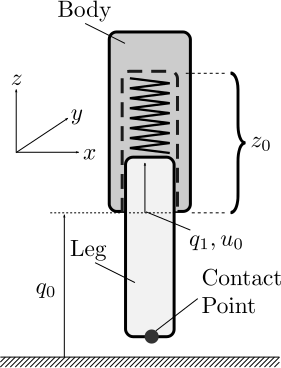
\includegraphics[width=0.25\textwidth]{./hoppingrobot}
	\end{center}
	\caption{One-legged Hopping Robot}
	\label{fig:hoppingrobot}
\end{wrapfigure}

Martin Felis (martin.felis@iwr.uni-heidelberg.de)

\bigskip
\bigskip

This is a simple example that should get you started with MUSCOD and RBDL. It is devoted to the introduction to contact forces and multi-phase optimal control problems. To this end we consider a simple one-legged hopping robot, see Figure \ref{fig:hoppingrobot}.

The hopping robot consists of two rigid bodies, the \emph{Body} and the
\emph{Leg}. The robot has two degrees of freedom:
\begin{itemize}
 \item $q_0$: the height (i.e. $Z$--coordinate) of the body \emph{Body}.
 \item $q_1$: the retraction of the body \emph{Leg}.
\end{itemize}
The two elements bodies are connected by a prismatic joint and a spring.
In the case of maximal extension of the leg, i.e. $q_1 = 0$, the spring
is fully extended to length $z_0$. The translation of the robot's leg can
be controlled by the linear force in the control $u_0$. 

In addition to gravity and interior forces of the actuated joints, it is
important to also model external ground reaction forces during the contact
phase. Furthermore, we want to be able to model contact gains due to
collisions. 

Here, the collision is modeled as an instantaneous event that results in
discontinuities in the velocities. In \muscod{} this can be modeled using
``Transition Phases'' that have zero duration and are specified by using
the \texttt{def\_strans} pseudo-integrator in the DAT-file.

This leads to three different contact phases for the robot: the
\emph{flight} phase, the \emph{collision} transition phase, and the
\emph{contact} phase (see Figure \ref{fig:phase_overview}).

\begin{wrapfigure}{l}{0.35\textwidth}
	\begin{center}
		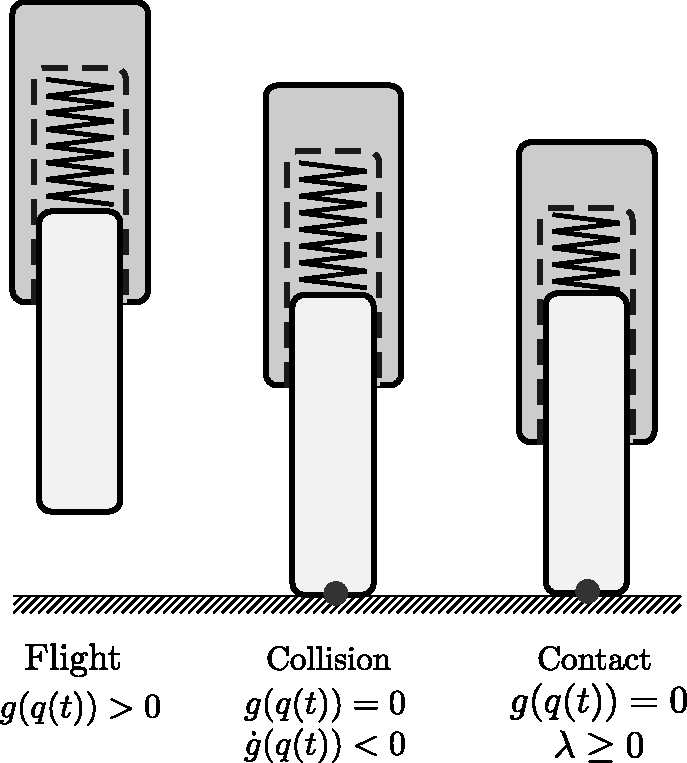
\includegraphics[width=0.35\textwidth]{./phase_overview}
	\end{center}
	\caption{Overview of the three phases}
	\label{fig:phase_overview}
\end{wrapfigure}

The three different phases a characterized by the following properties:

\paragraph{Flight Phase:} There is no contact with the ground ($g(q(t)) > 0$) and there are no external forces.

\paragraph{Collision Transition Phase:} The contact condition $g(q(t))
= 0$ is fulfilled. In addition, the contact point is moving along the
negative contact normal. Note, that collisions in general result in
discontinuities in the velocity variables.

\paragraph{Contact Phase:}The contact condition $g(q(t)) = 0$ is fulfilled and there are positive ground reaction forces $\lambda$ in the direction of the contact normal.

All phases can be modeled using \rbdl{}. For details we refer to the official documentation (Section "`External Contacts"').

\clearpage

\subsection*{Tasks}

Determine an optimal control, such that the robot performs a periodic motion with a (vertical) velocity of $v > 5$ at take of.

\begin{enumerate}
	\item Define the model name and the correct integrators for the individual phases in the
		DAT-file (\verb$libind$).
	\item Complete the function \verb$update_generalized_variables$ that
		copy the values from the \verb$double$ arrays to the correct Eigen
		vectors \verb$Q, QDot, Tau$ that are then used by \rbdl{} methods.
	\item Complete the right-hand side function stubs \verb$ffcn_flight$, \verb$ffcn_touchdown$,
		\verb$ffcn_contact$.
	\item Define the point constraints \verb$rdfcn_*$ and 
		\verb$def_mpc()$.
	\item Optimization 1: Minimize the applied force $u_0$ during the whole
		process.
	\item Optimization 2: Minimize the collision impact.
\end{enumerate}
\medskip

\end{document}
